\section{Appendix}

\subsection{Tables}

% statistical description for the chemical data within reference, intermediate, and degraded sites based on PCA assessment
% Table 1: Major Metals
\begin{table}[ht]
\centering
\caption{Descriptive Statistics of Major Metals by Site Label}
\label{tab:chem_desc_metals}
\begin{tabular}{>{\centering\arraybackslash}m{2.5cm} >{\centering\arraybackslash}m{1.5cm} >{\centering\arraybackslash}m{2cm} >{\centering\arraybackslash}m{2cm} >{\centering\arraybackslash}m{2cm}}
\toprule
 & \textbf{SumReal} & \textbf{degraded} & \textbf{intermediate} & \textbf{reference} \\
\midrule
\multirow[t]{2}{*}{Al} & mean & 4276.423 & 6380.140 & 4319.381 \\
 & std & 2888.769 & 5523.949 & 1767.861 \\
\cline{1-5}
\multirow[t]{2}{*}{As} & mean & 2.186 & 1.777 & 2.232 \\
 & std & 1.602 & 1.290 & 1.041 \\
\cline{1-5}
\multirow[t]{2}{*}{Bi} & mean & 17.085 & 17.505 & 17.622 \\
 & std & 10.352 & 10.273 & 9.722 \\
\cline{1-5}
\multirow[t]{2}{*}{Ca} & mean & 28180.500 & 33518.930 & 28480.714 \\
 & std & 14031.433 & 11400.266 & 11870.107 \\
\cline{1-5}
\multirow[t]{2}{*}{Cd} & mean & 0.535 & 0.351 & 0.271 \\
 & std & 0.649 & 0.202 & 0.233 \\
\cline{1-5}
\multirow[t]{2}{*}{Co} & mean & 4.049 & 4.497 & 3.984 \\
 & std & 1.733 & 2.209 & 1.118 \\
\cline{1-5}
\multirow[t]{2}{*}{Cr} & mean & 13.254 & 12.830 & 9.007 \\
 & std & 16.373 & 11.835 & 2.937 \\
\cline{1-5}
\multirow[t]{2}{*}{Cu} & mean & 16.958 & 18.082 & 12.946 \\
 & std & 22.388 & 29.120 & 9.003 \\
\cline{1-5}
\multirow[t]{2}{*}{Fe} & mean & 9495.000 & 11246.789 & 9650.905 \\
 & std & 5392.824 & 6804.654 & 3856.739 \\
\cline{1-5}
\multirow[t]{2}{*}{Hg} & mean & 0.474 & 0.324 & 0.196 \\
 & std & 1.230 & 0.420 & 0.365 \\
\cline{1-5}
\multirow[t]{2}{*}{K} & mean & 818.927 & 1285.558 & 845.657 \\
 & std & 638.053 & 1092.550 & 411.332 \\
\cline{1-5}
\multirow[t]{2}{*}{Mg} & mean & 12849.500 & 15204.175 & 12269.143 \\
 & std & 6104.202 & 5764.037 & 5281.794 \\
\cline{1-5}
\multirow[t]{2}{*}{Mn} & mean & 161.228 & 188.900 & 161.905 \\
 & std & 76.973 & 86.663 & 57.883 \\
\cline{1-5}
\multirow[t]{2}{*}{Na} & mean & 118.998 & 134.042 & 123.611 \\
 & std & 49.081 & 43.693 & 41.021 \\
\cline{1-5}
\multirow[t]{2}{*}{Ni} & mean & 11.225 & 12.399 & 9.136 \\
 & std & 8.851 & 8.424 & 3.542 \\
\cline{1-5}
\multirow[t]{2}{*}{Pb} & mean & 12.515 & 8.774 & 8.573 \\
 & std & 32.312 & 22.204 & 18.750 \\
\cline{1-5}
\multirow[t]{2}{*}{Sb} & mean & 17.262 & 16.765 & 18.001 \\
 & std & 11.879 & 13.115 & 13.743 \\
\cline{1-5}
\multirow[t]{2}{*}{V} & mean & 15.274 & 18.353 & 15.183 \\
 & std & 7.012 & 9.560 & 4.408 \\
\cline{1-5}
\multirow[t]{2}{*}{Zn} & mean & 52.732 & 46.181 & 35.677 \\
 & std & 48.896 & 44.586 & 17.938 \\
\cline{1-5}
\bottomrule
\end{tabular}
\end{table}

% Table 2: Organic Carbon and Chlorinated Benzenes
\begin{table}[ht]
\centering
\caption{Descriptive Statistics of Organic Carbon and Chlorinated Benzenes}
\label{tab:chem_desc_organics}
\begin{tabular}{>{\centering\arraybackslash}m{2.5cm} >{\centering\arraybackslash}m{1.5cm} >{\centering\arraybackslash}m{2cm} >{\centering\arraybackslash}m{2cm} >{\centering\arraybackslash}m{2cm}}
\toprule
 & \textbf{SumReal} & \textbf{degraded} & \textbf{intermediate} & \textbf{reference} \\
\midrule
\multirow[t]{2}{*}{\%OC} & mean & 2.110 & 2.405 & 1.779 \\
 & std & 1.599 & 1.458 & 0.682 \\
\cline{1-5}
\multirow[t]{2}{*}{1245-TCB} & mean & 0.906 & 1.201 & 0.555 \\
 & std & 2.321 & 2.143 & 1.035 \\
\cline{1-5}
\multirow[t]{2}{*}{1234-TCB} & mean & 0.252 & 0.234 & 0.253 \\
 & std & 0.257 & 0.240 & 0.332 \\
\cline{1-5}
\multirow[t]{2}{*}{QCB} & mean & 0.729 & 1.255 & 0.636 \\
 & std & 1.015 & 3.055 & 0.871 \\
\cline{1-5}
\multirow[t]{2}{*}{HCB} & mean & 2.759 & 17.713 & 2.904 \\
 & std & 4.291 & 83.487 & 6.011 \\
\cline{1-5}
\multirow[t]{2}{*}{OCS} & mean & 1.213 & 1.502 & 0.721 \\
 & std & 3.395 & 3.606 & 1.874 \\
\cline{1-5}
\bottomrule
\end{tabular}
\end{table}

% Table 3: Pesticides and PCBs
\begin{table}[ht]
\centering
\caption{Descriptive Statistics of Pesticides and PCBs}
\label{tab:chem_desc_pesticides}
\begin{tabular}{>{\centering\arraybackslash}m{2.5cm} >{\centering\arraybackslash}m{1.5cm} >{\centering\arraybackslash}m{2cm} >{\centering\arraybackslash}m{2cm} >{\centering\arraybackslash}m{2cm}}
\toprule
 & \textbf{SumReal} & \textbf{degraded} & \textbf{intermediate} & \textbf{reference} \\
\midrule
\multirow[t]{2}{*}{p,p'-DDE} & mean & 0.679 & 0.485 & 0.324 \\
 & std & 1.255 & 0.930 & 0.328 \\
\cline{1-5}
\multirow[t]{2}{*}{p,p'-DDD} & mean & 3.879 & 0.772 & 0.862 \\
 & std & 14.634 & 1.039 & 0.923 \\
\cline{1-5}
\multirow[t]{2}{*}{mirex} & mean & 0.253 & 0.212 & 0.134 \\
 & std & 0.682 & 0.332 & 0.242 \\
\cline{1-5}
\multirow[t]{2}{*}{Heptachlor Epoxide} & mean & 0.098 & 0.051 & 0.071 \\
 & std & 0.235 & 0.250 & 0.211 \\
\cline{1-5}
\multirow[t]{2}{*}{total PCB} & mean & 15.137 & 10.705 & 7.715 \\
 & std & 32.189 & 36.285 & 16.795 \\
\cline{1-5}
\bottomrule
\end{tabular}
\end{table}

\clearpage
\subsection{Figures}

\begin{figure}[!h]
    \centering
    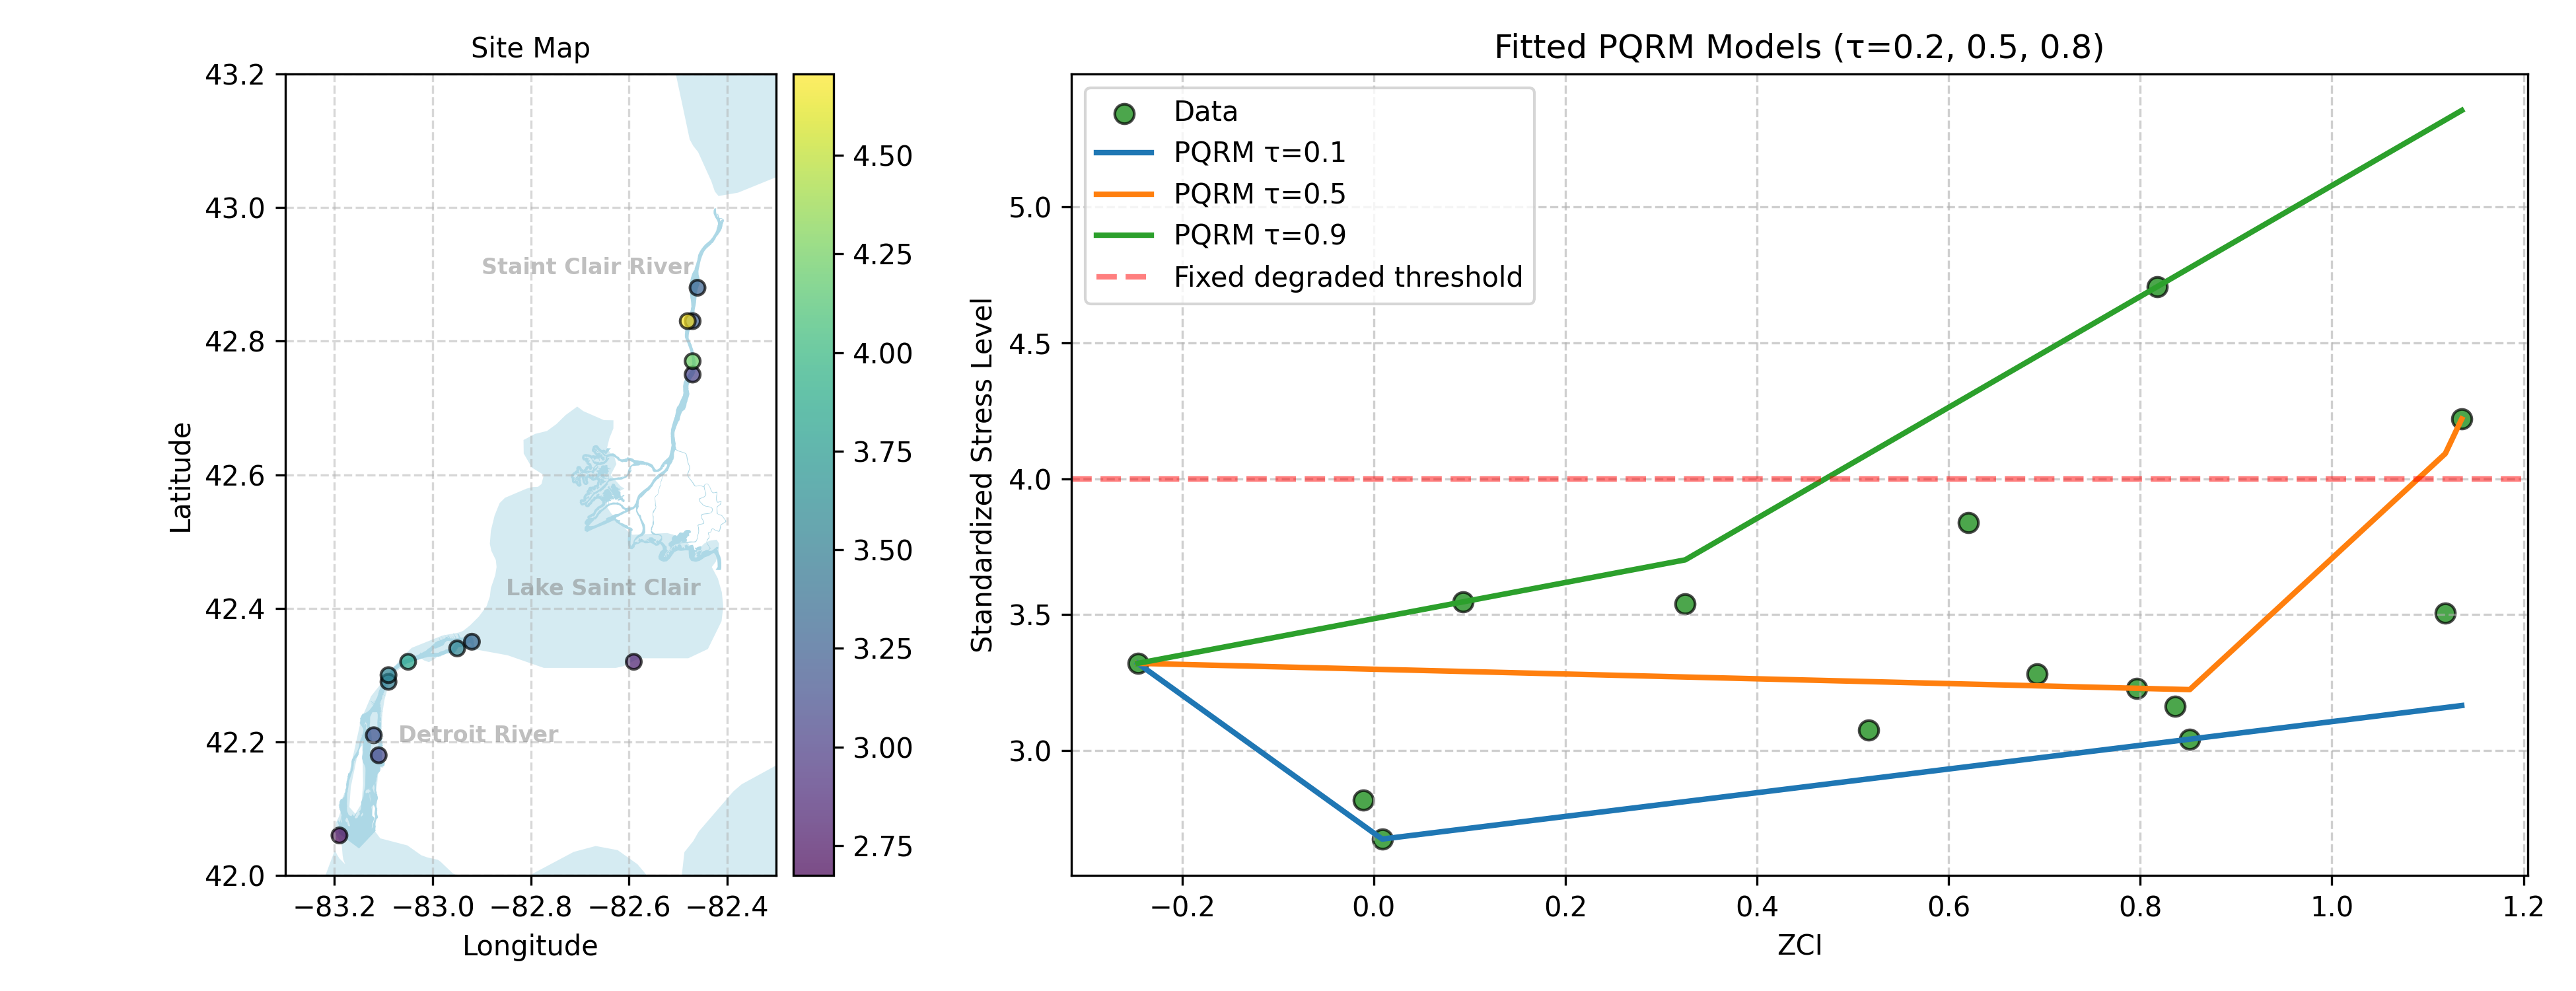
\includegraphics[width=0.8\textwidth]{../results/preliminary_results/pqrm_quantile_regression_pattern_1.png}
    \caption{Piecewise Quantile Regression for cluster 1}
    \label{fig:pqrm_quantile_regression_pattern_1}
\end{figure}

\begin{figure}[!h]
    \centering
    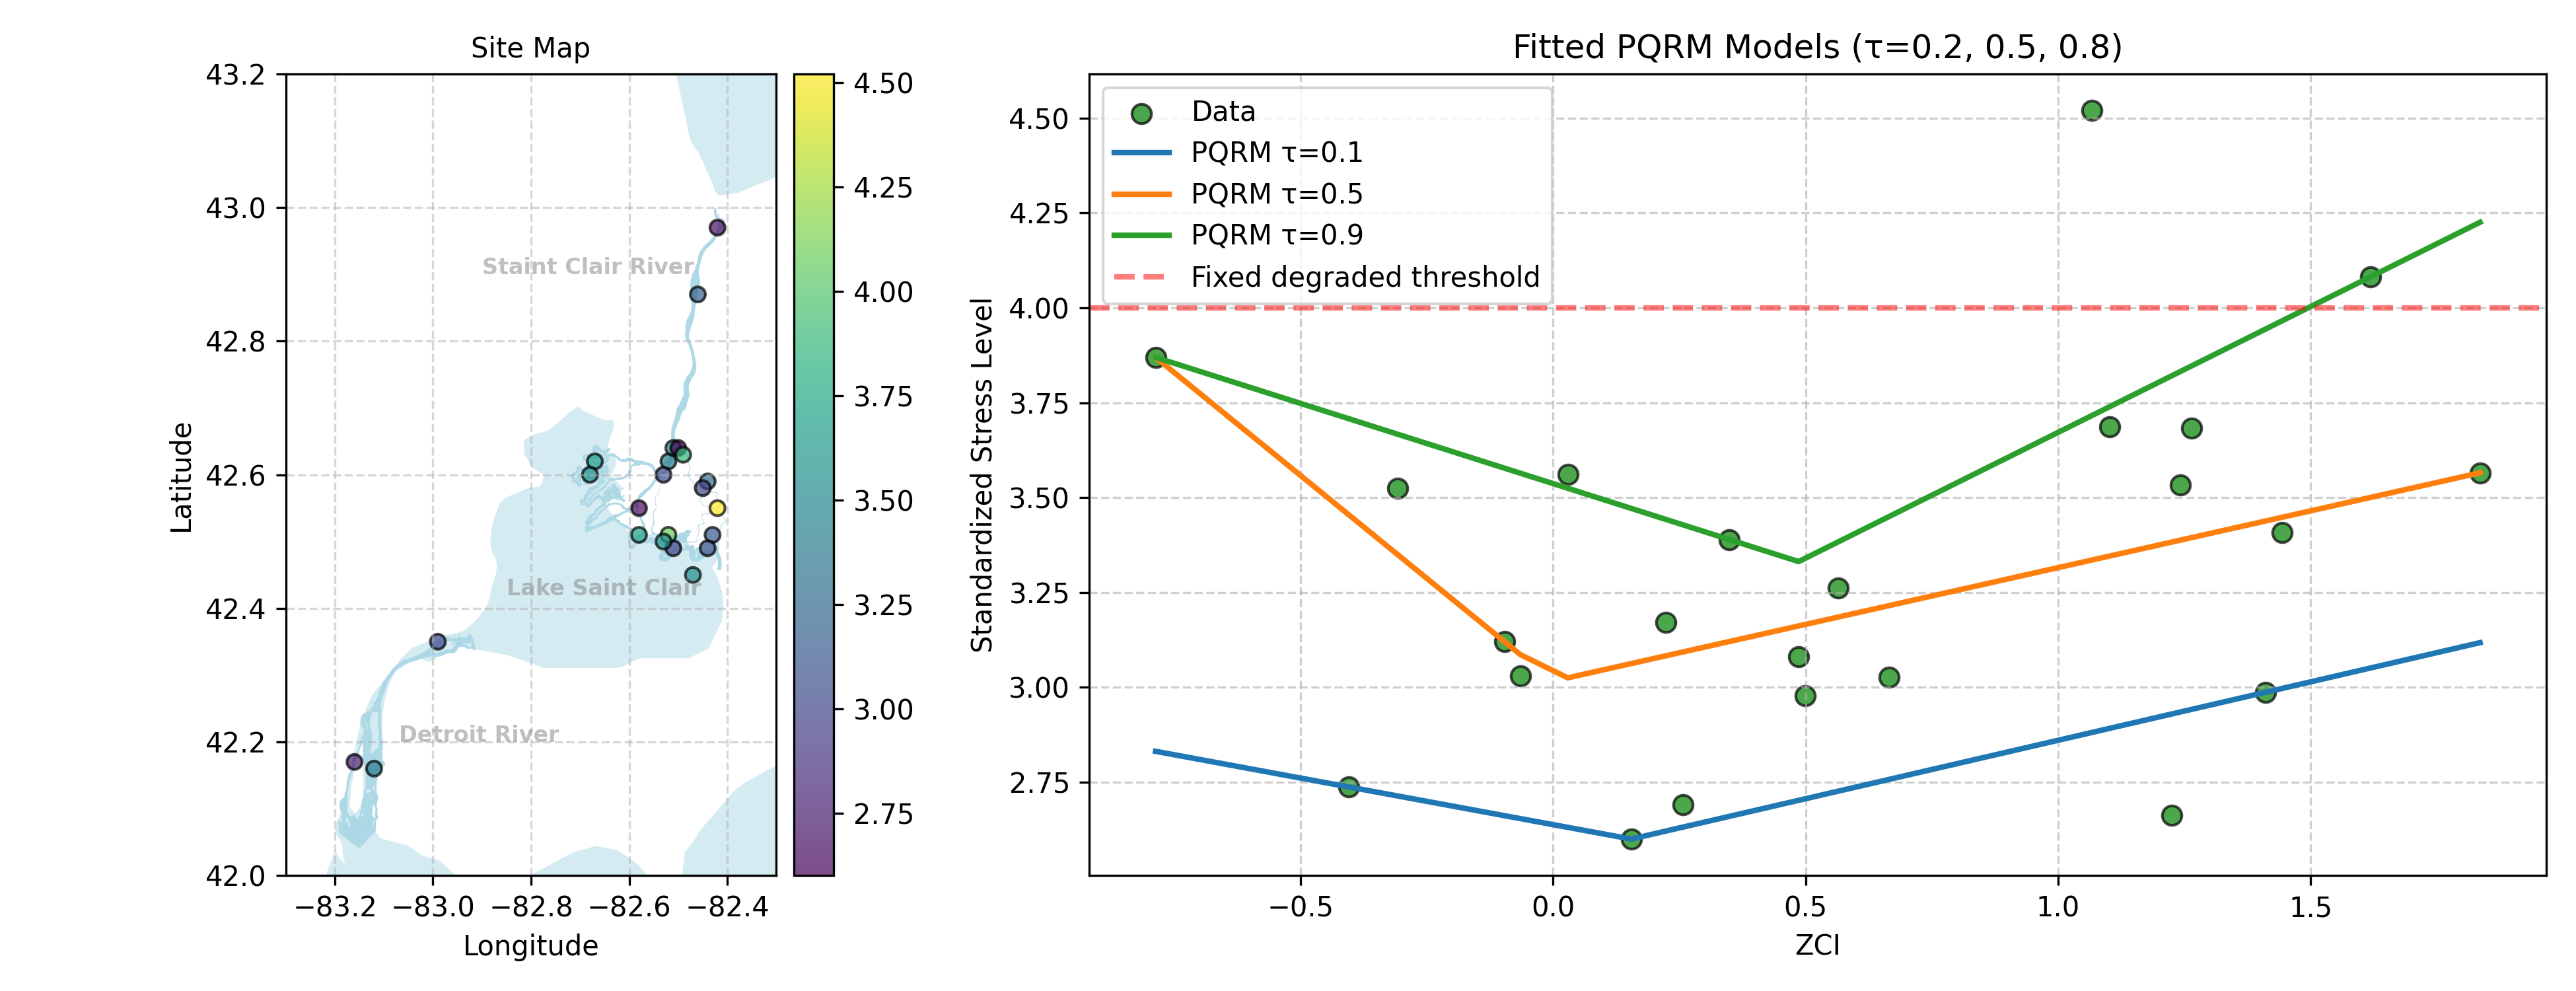
\includegraphics[width=0.8\textwidth]{../results/preliminary_results/pqrm_quantile_regression_pattern_2.png}
    \caption{Piecewise Quantile Regression for cluster 2}
    \label{fig:pqrm_quantile_regression_pattern_2}
\end{figure}

\begin{figure}[!h]
    \centering
    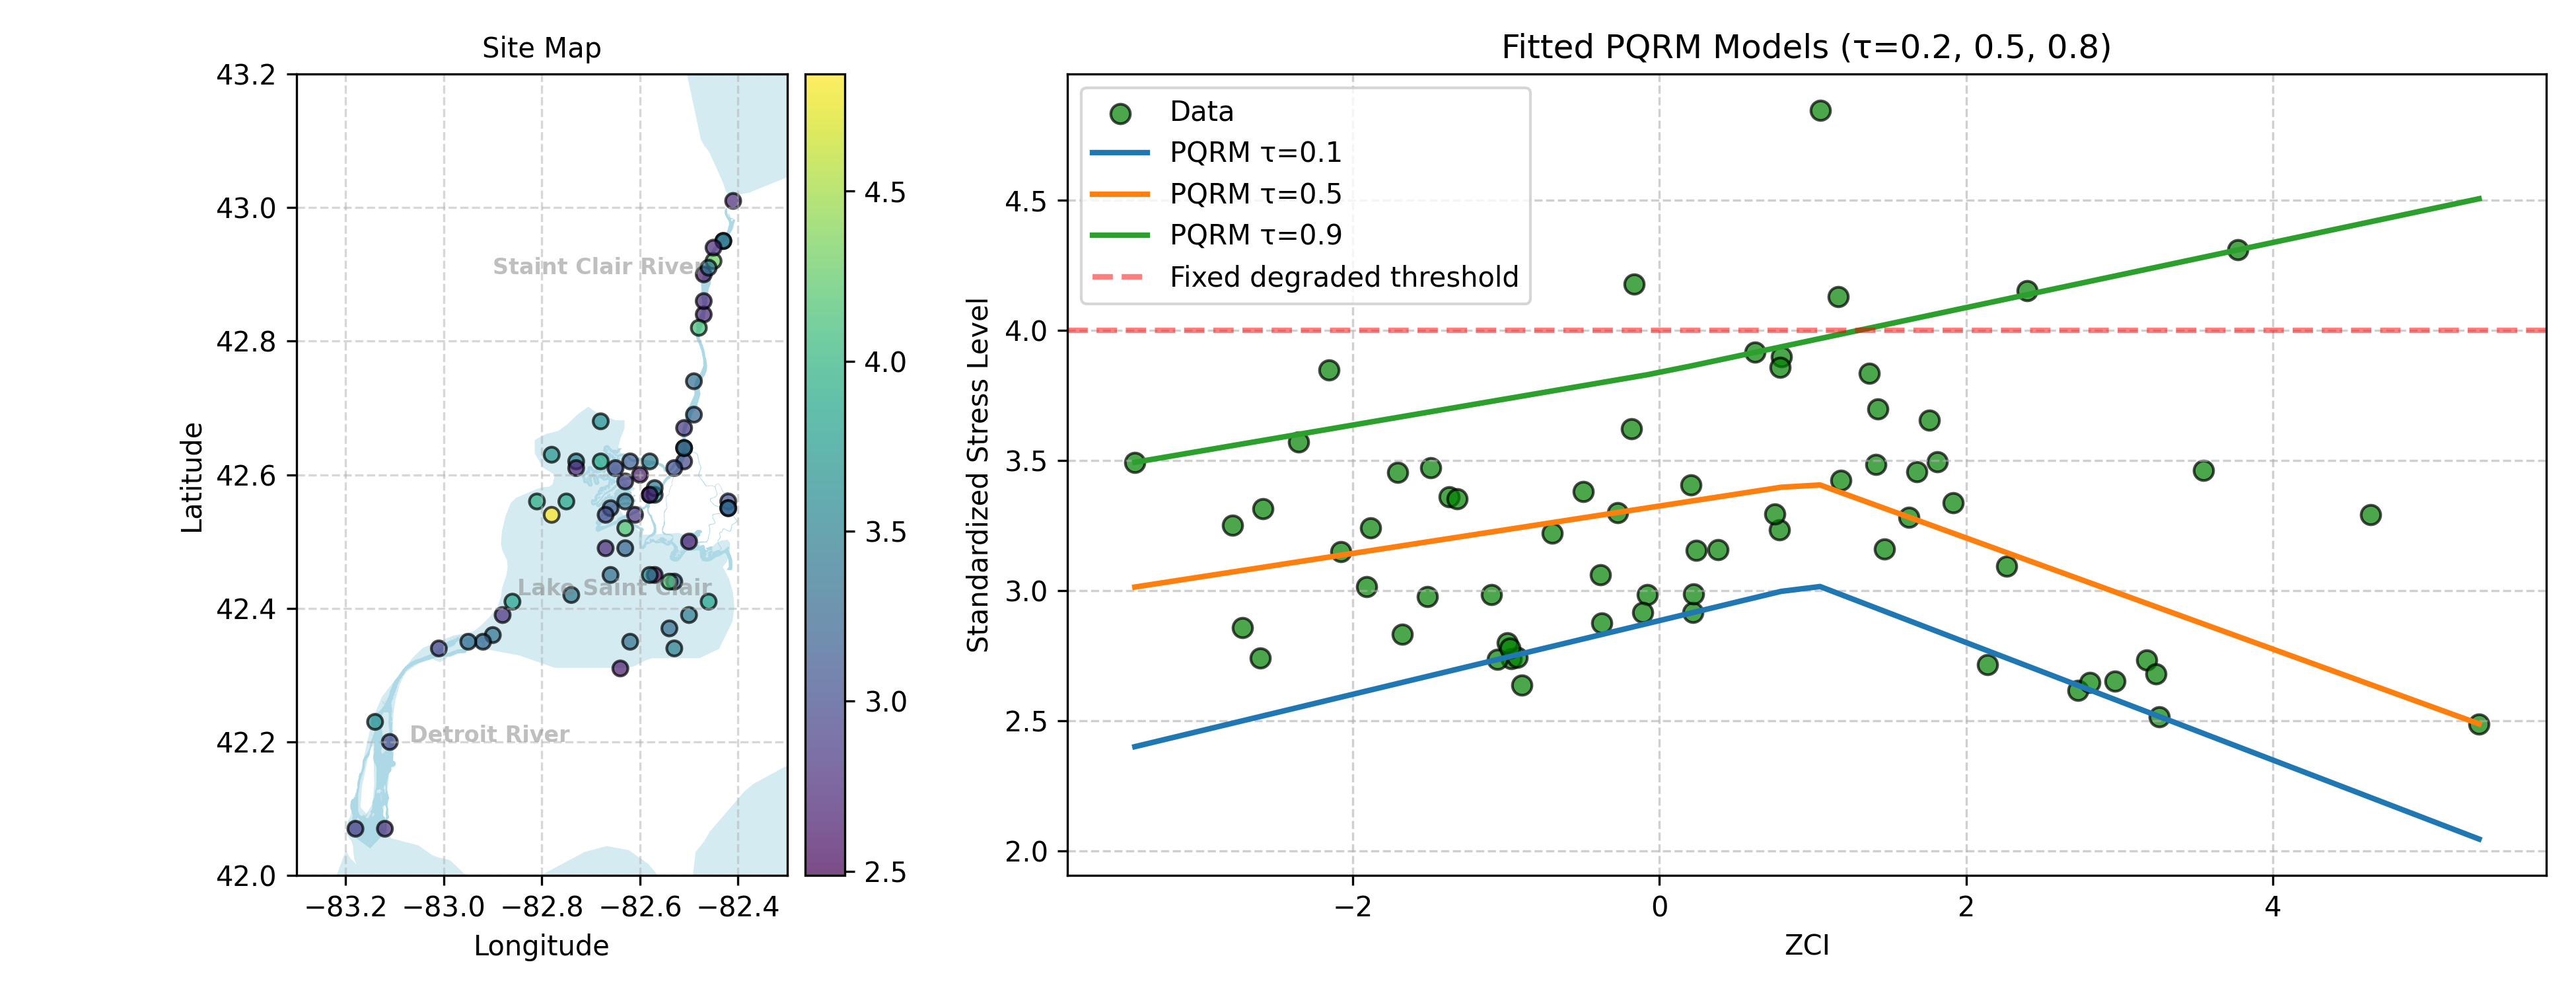
\includegraphics[width=0.8\textwidth]{../results/preliminary_results/pqrm_quantile_regression_pattern_3.png}
    \caption{Piecewise Quantile Regression for cluster 3}
    \label{fig:pqrm_quantile_regression_pattern_3}
\end{figure}

\begin{figure}[!h]
    \centering
    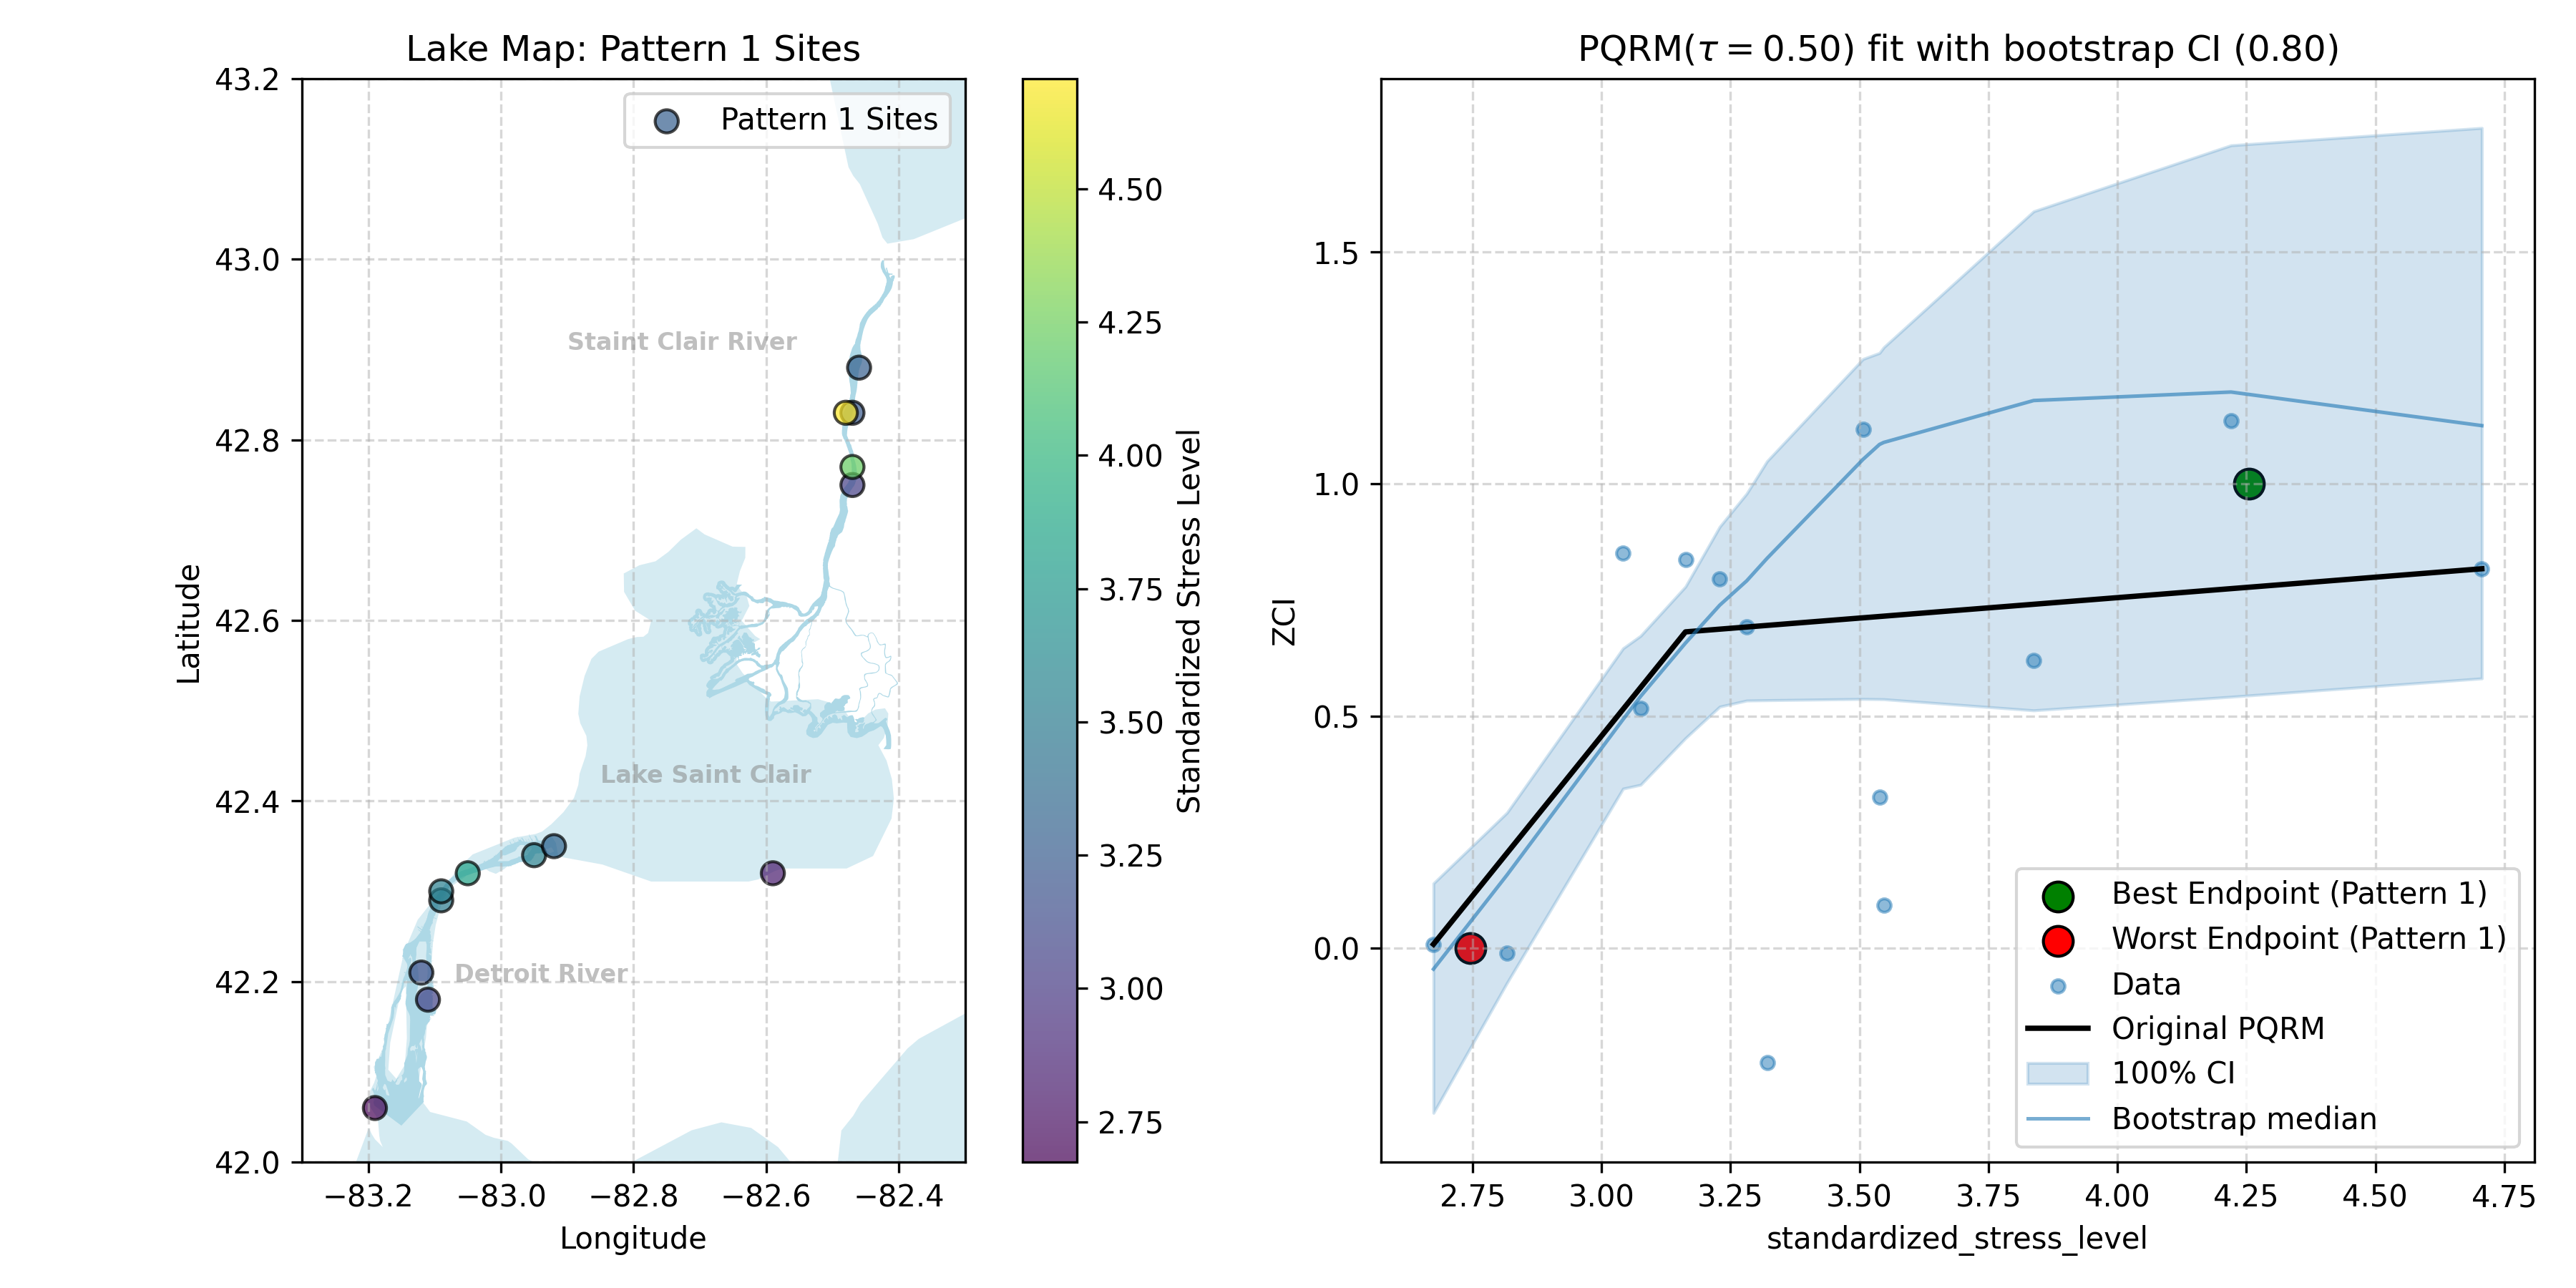
\includegraphics[width=0.8\textwidth]{../results/preliminary_results/pqrm_pattern_1_tau_0.5.png}
    \caption{Piecewise Quantile Regression for cluster 1 with inference of confidence intervals}
    \label{fig:pqrm_pattern_1_tau_0.5}
\end{figure}

\begin{figure}[!h]
    \centering
    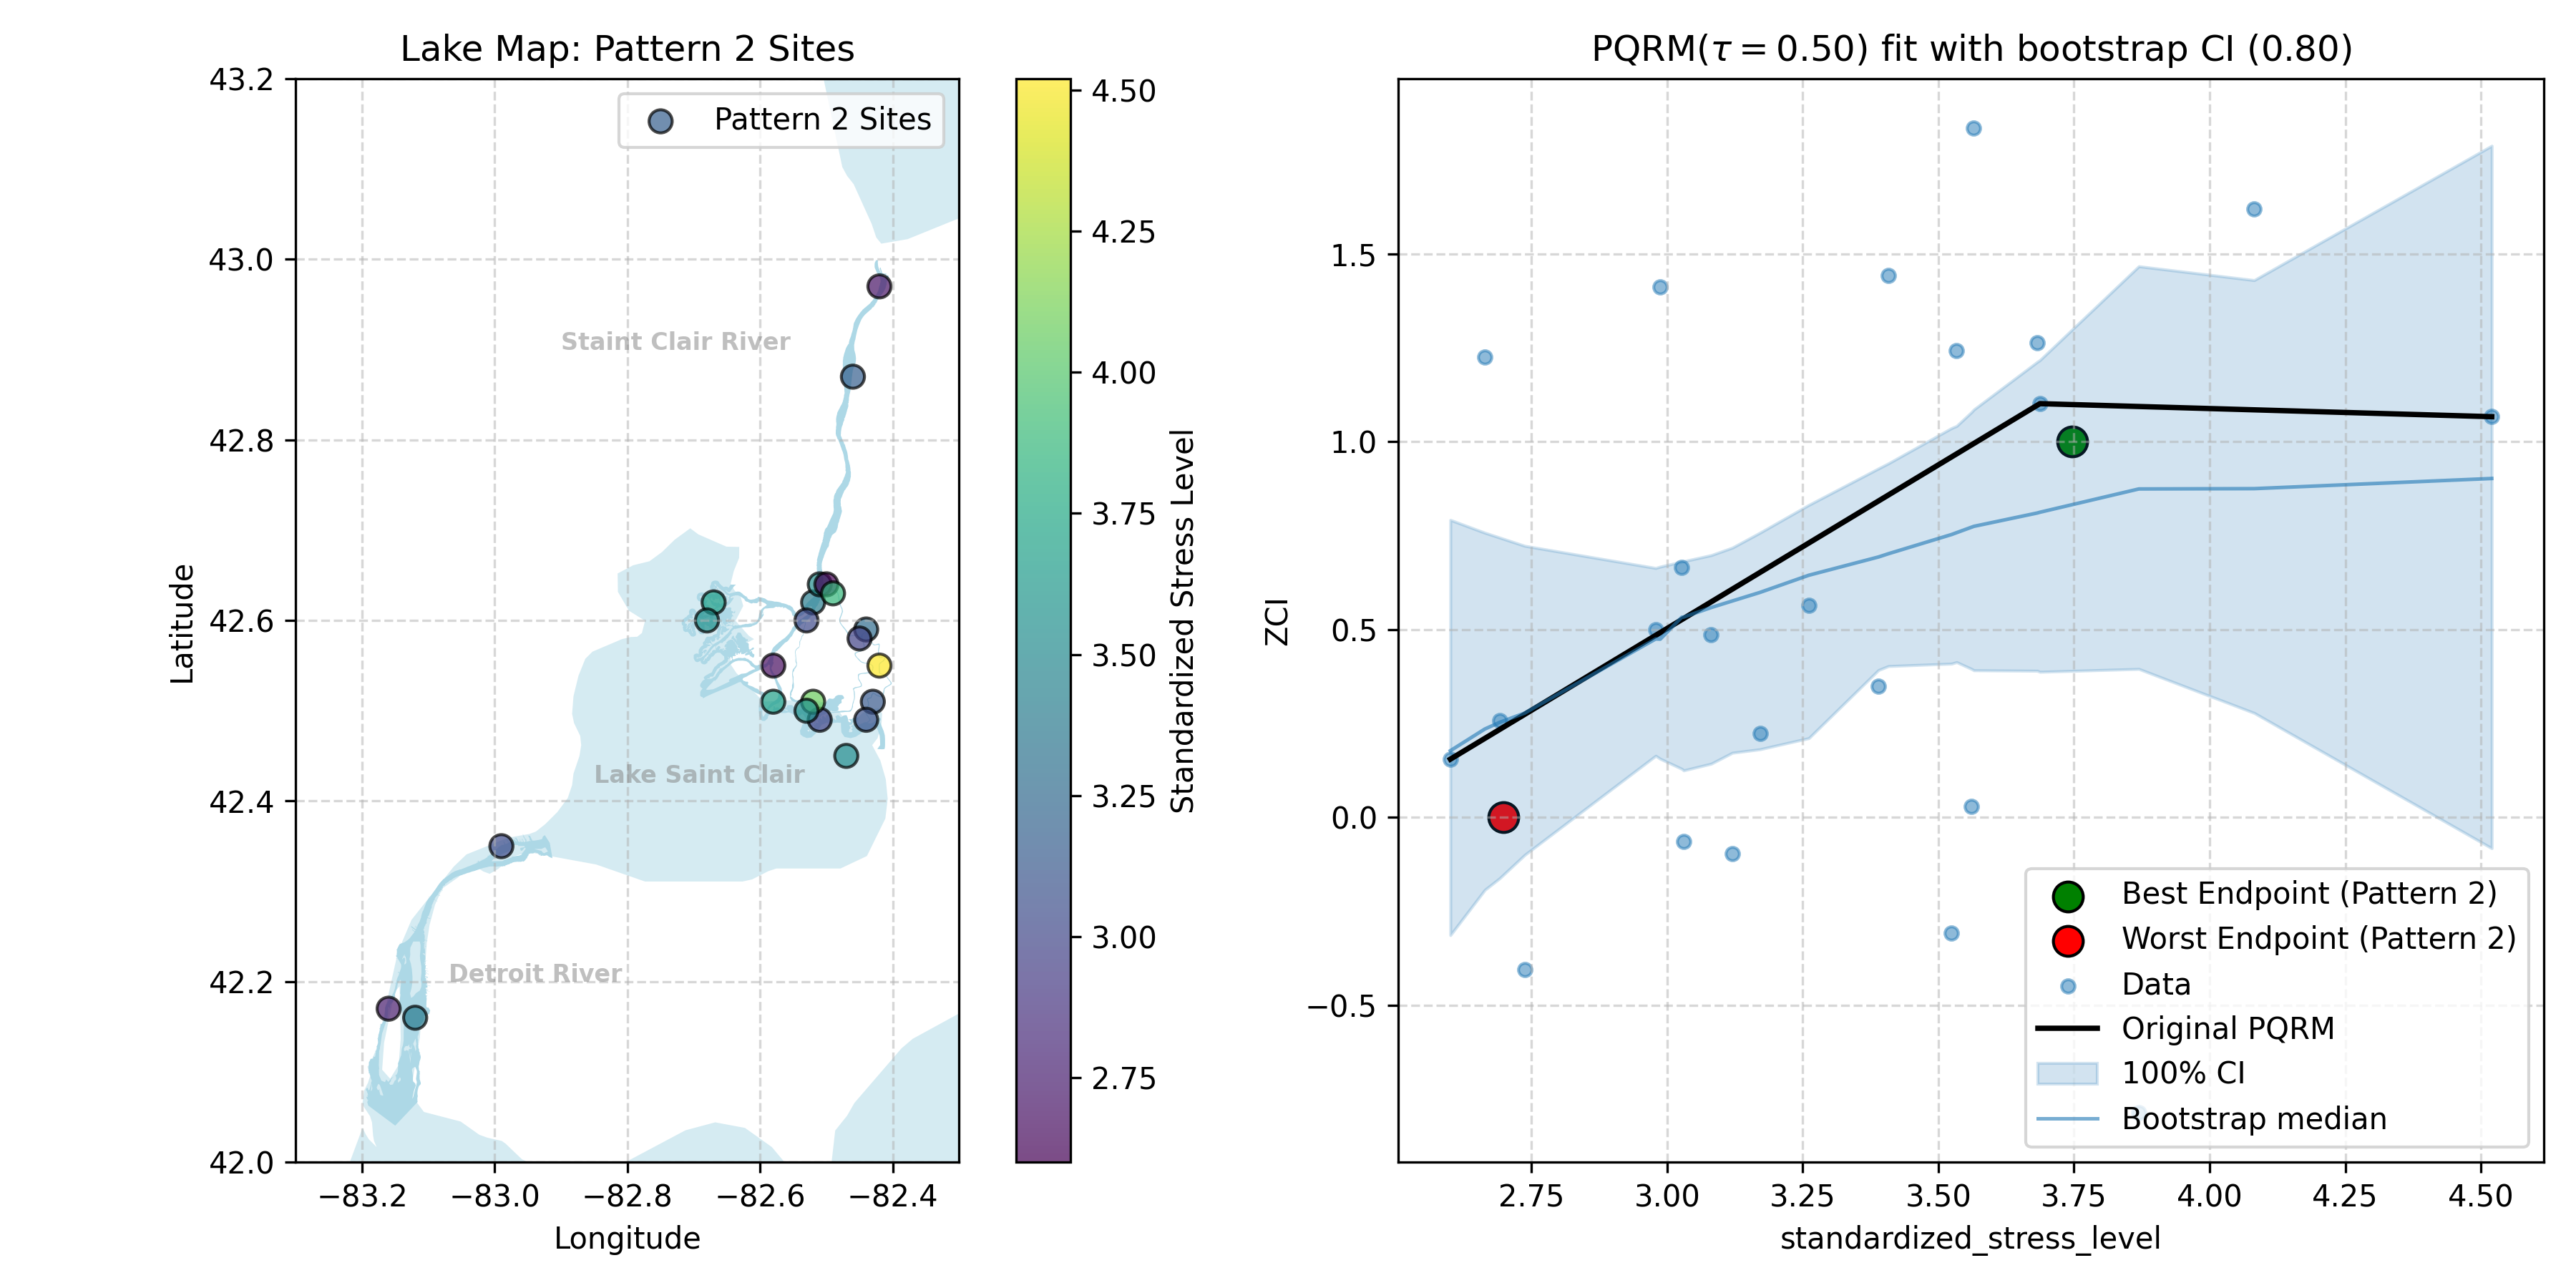
\includegraphics[width=0.8\textwidth]{../results/preliminary_results/pqrm_pattern_2_tau_0.5.png}
    \caption{Piecewise Quantile Regression for cluster 2 with inference of confidence intervals}
    \label{fig:pqrm_pattern_2_tau_0.5}
\end{figure}

\begin{figure}[!h]
    \centering
    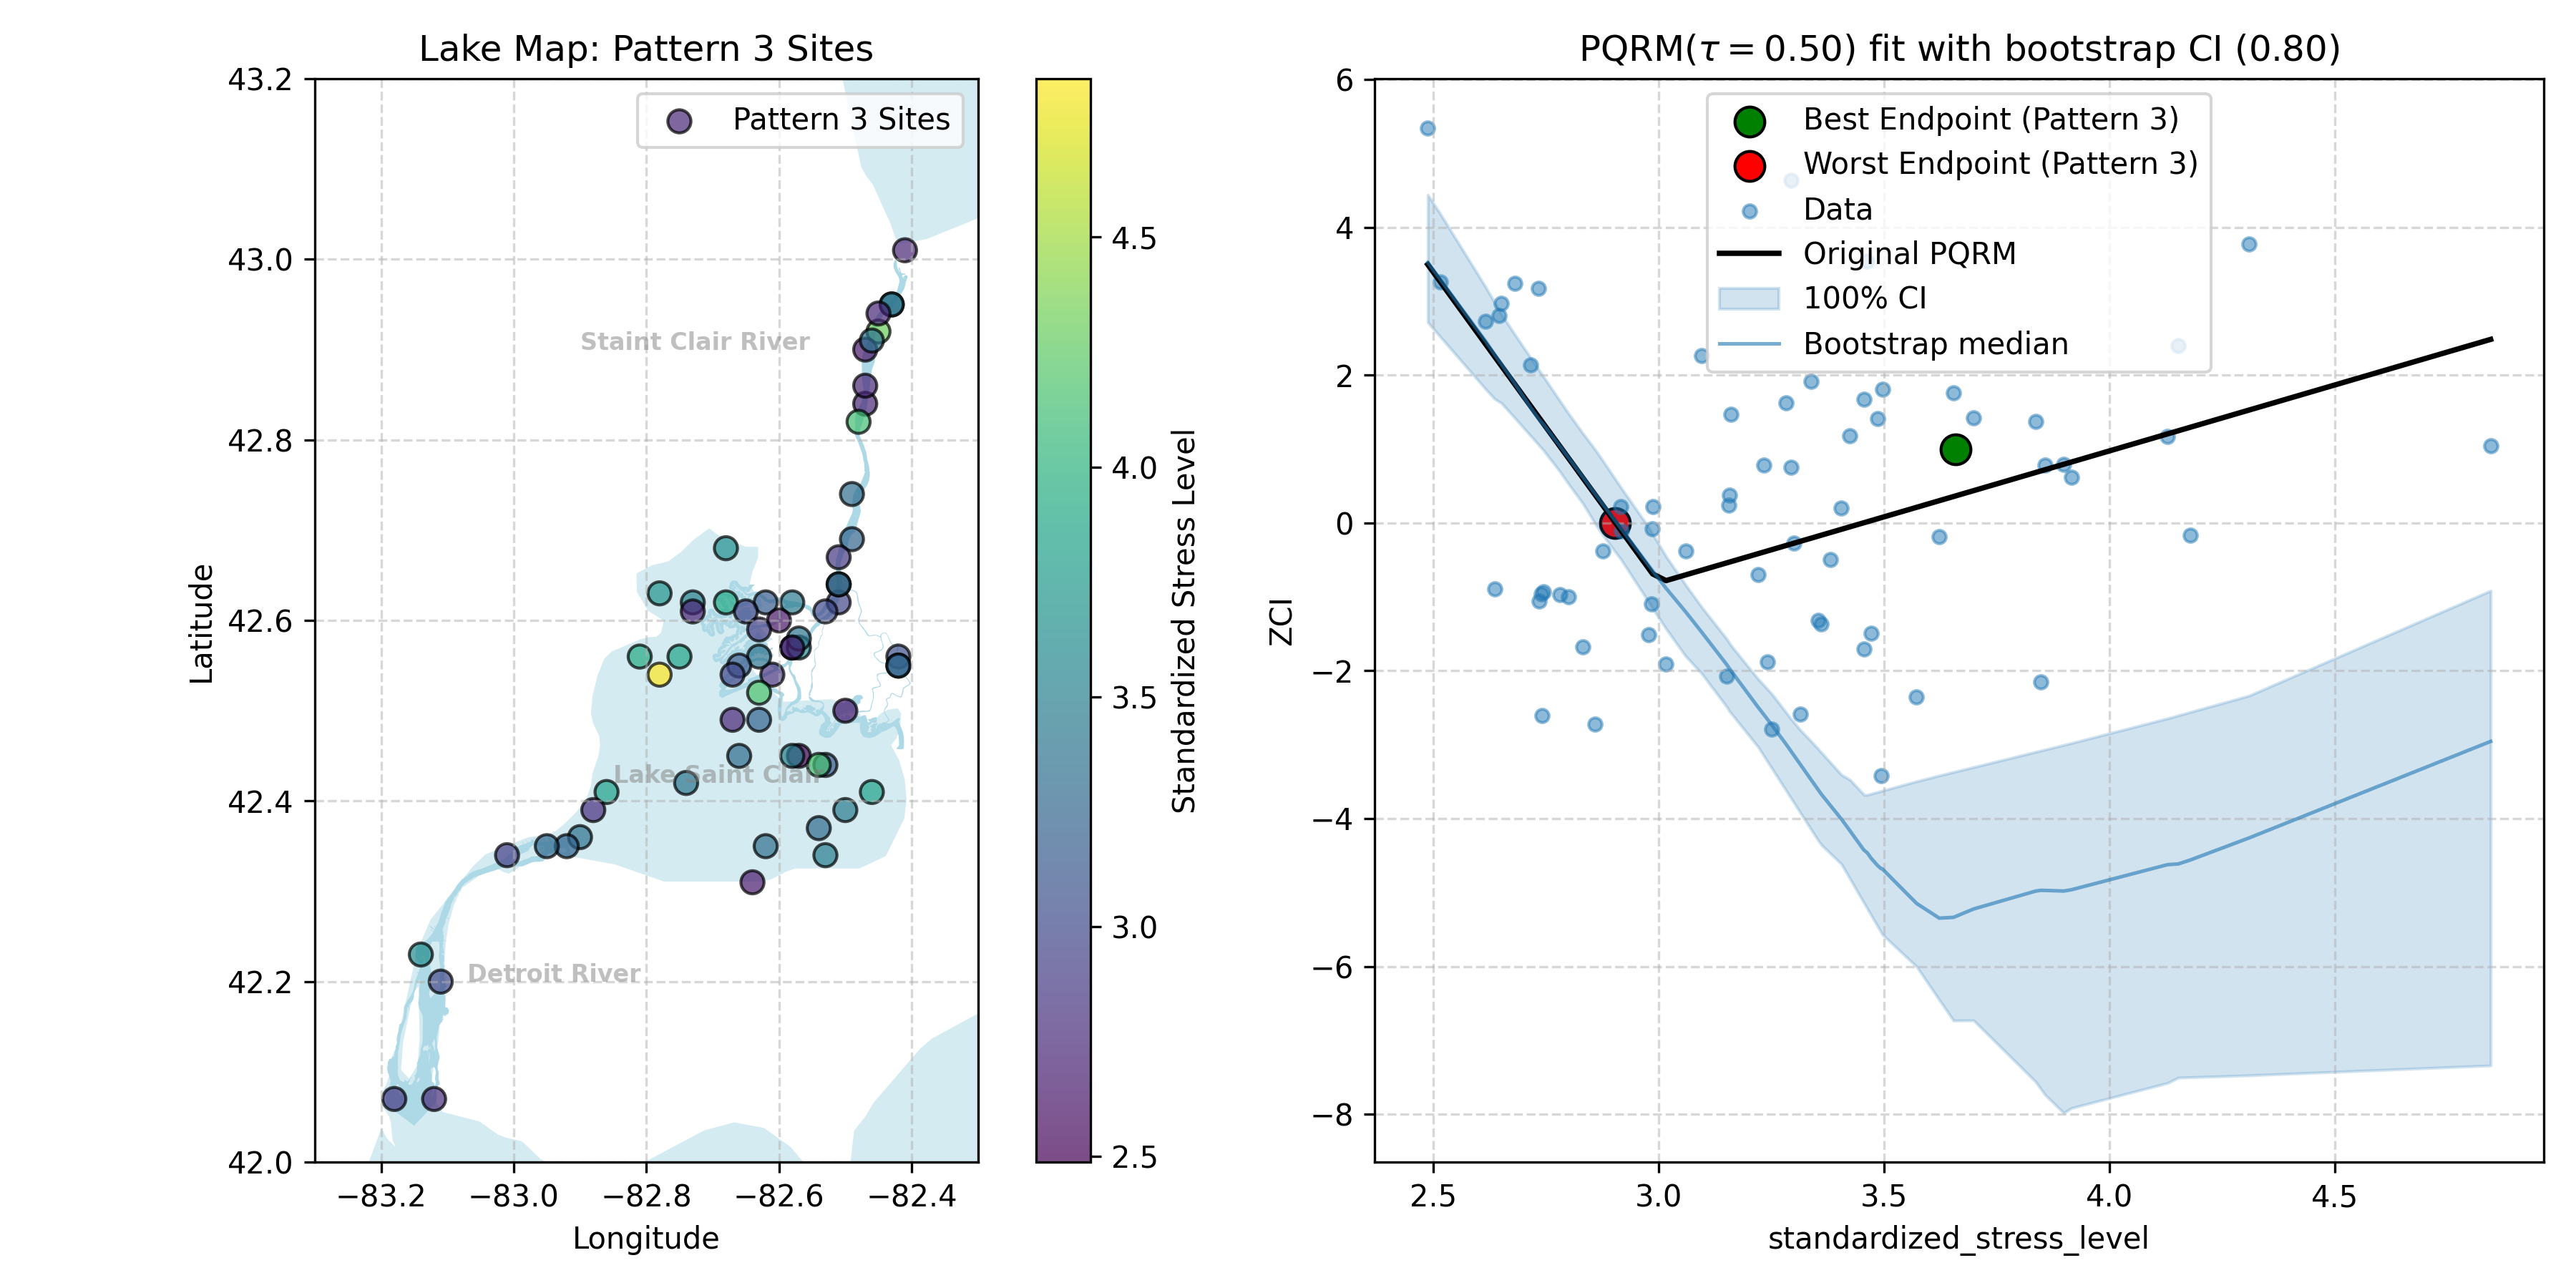
\includegraphics[width=0.8\textwidth]{../results/preliminary_results/pqrm_pattern_3_tau_0.5.png}
    \caption{Piecewise Quantile Regression for cluster 3 with inference of confidence intervals}
    \label{fig:pqrm_pattern_3_tau_0.5}
\end{figure}

\begin{figure}[!h]
    \centering
    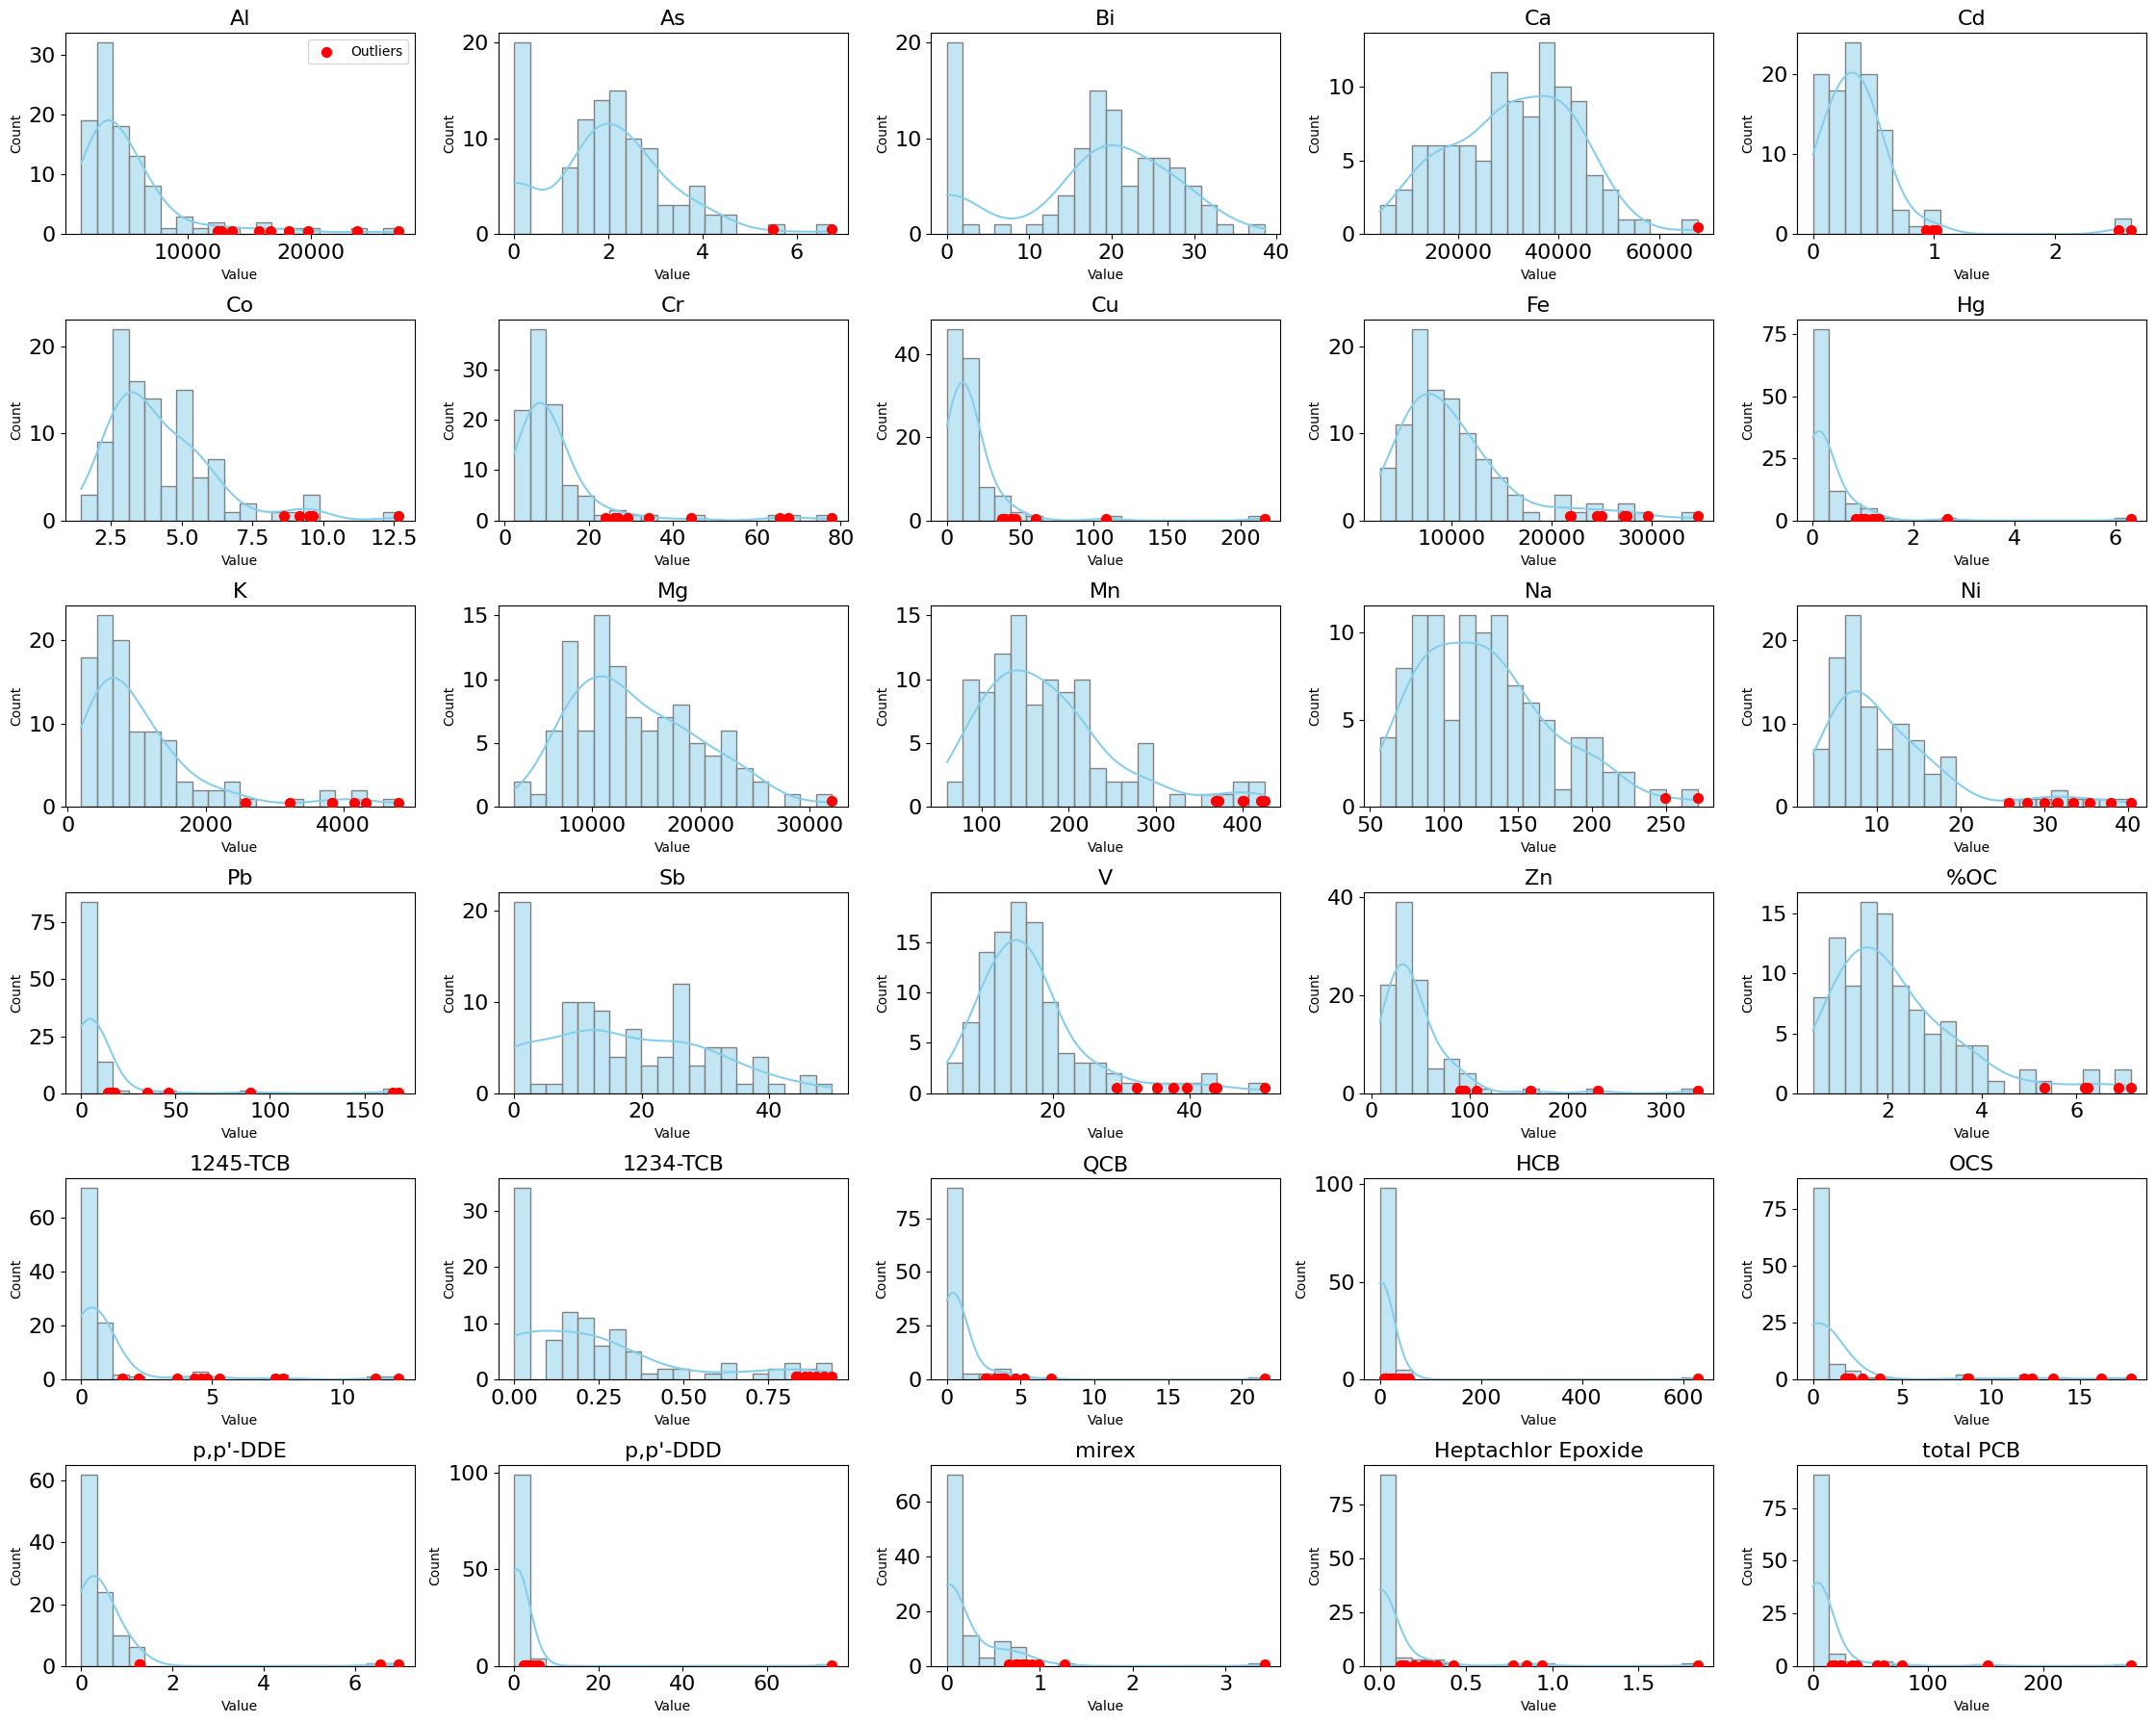
\includegraphics[width=0.8\textwidth]{../results/preliminary_results/raw_chemical_histgram.png}
    \caption{Example of outlier detection: Raw chemical histogram with IQR-detected outliers in red}
    \label{fig:raw_chemical_histgram}
\end{figure}

% \clearpage
% \subsection{Additional Math background supporting the major methods used in the program}

% \subsubsection{Principal Component Analysis for Sediment Contamination Assessment}

% In SVD, a data matrix $X$ is decomposed as $X = U \Sigma V^T$, where $U$ and $V$ are orthogonal matrices and
%  $\Sigma$ is a diagonal matrix of singular values.
% For PCA, the principal components correspond to
% the directions of maximum variance, which are given by the right singular vectors in $V$.
% By incorporating weights into the data matrix, Weighted PCA modifies the SVD process 
% to emphasize certain observations(row or column), allowing for more flexible dimensionality reduction 
% tailored to the importance of each data point.

% Given a data matrix $X \in \mathbb{R}^{m \times n}$, the SVD decomposes $X$ as $X = U \Sigma V^T$, where:
% \begin{itemize}
%     \item $U \in \mathbb{R}^{m \times m}$ contains the left singular vectors (columns),
%     \item $\Sigma \in \mathbb{R}^{m \times n}$ is a diagonal matrix of singular values,
%     \item $V \in \mathbb{R}^{n \times n}$ contains the right singular vectors (columns).
% \end{itemize}

% To solve for $U$ and $V$:
% \begin{enumerate}
%     \item Compute $X^T X$ and find its eigenvectors and eigenvalues. The eigenvectors form the columns of $V$.
%     \item It can be proven that \(\mu_i^T = \frac{X v_i}{\sigma_i}\) is the $i$-th column of $U$, where $\sigma_i$ is the $i$-th singular value(square root of eigenvalue \(\lambda_i\)).
%     \item The singular values in $\Sigma$ are the square roots of the nonzero eigenvalues from either $X X^T$ or $X^T X$.
% \end{enumerate}

% Mathematically, given a matrix $X$ of shape $(m, n)$, the SVD can be expressed as: 
% \[
% (X^T X) V = V \Lambda, \quad \Lambda = \text{diag}(\lambda_1, \lambda_2, \ldots, \lambda_n)
% \]
% According to spectral theorem, the eigenvalues $\lambda_i$ are non-negative and can be ordered as $\lambda_1 \geq \lambda_2 \geq \ldots \geq \lambda_n \geq 0$.
% \(V\) is an orthogonal matrix, meaning \(V^T V = I\), where \(I\) is the identity matrix.
% It gives:
% \[
% (X^T X) = V \Lambda V^T
% \]
% To a centered sample matrix of size \(m\) with \(n\) features, its covariance matrix is \(\frac{1}{m-1} (X^T X)\).
% Via the eigenvalue decomposition, the variation in it can be expressed by the paris of eigenvalues and eigenvectors,
% which are a series of rank-one matrices that carry different and independent information:
% \[
% \frac{1}{m-1} (X^T X) = \frac{1}{m-1} \sum_{i=1}^{n} \lambda_i v_i v_i^T
% \]

% Therefore, when columns in \(X\) represent different features, the columns \(v_i\) of \(V\) are the principal components 
% that have its values as the linear combinations of the original features, and the scaled eigenvalues \(\frac{\lambda_i}{m-1}\)
% as the amount of variation explained by each principal component.

% Weighted PCA leverages the Singular Value Decomposition (SVD)
% to extract principal components from weighted data.

% \subsubsection{Hierarchical Clustering analysis for Taxa Community Structure Analysis}

% Hierarchical clustering offers a data-driven approach to group sampling sites based on environmental or 
% community-level similarities. Unlike partitioning methods, hierarchical clustering builds a nested tree
% (dendrogram) that captures the progressive grouping of observations based on their dissimilarities.
% In the context of my program, hierarchical clustering can be leveraged to define natural environmental 
% classes prior to modeling the biological response to stressors.

% Let each observation \( x_i \in \mathbb{R}^p \) denote a site with p-dimensional attributes (e.g., environmental variables). 
% The dissimilarity between two observations \( x_i \) and \( x_{i'} \) is measured by a distance function,
% often chosen as the squared Euclidean distance:
% \[ d(x_i, x_{i'}) = \sum_{j=1}^p (x_{ij} - x_{i'j})^2 \]

% Based on the distance metric, we can define the similarity measure on variable and observation levels as the following:
% \[
% \begin{aligned}
%     &\text{Variable level:} \quad d_j(x_{ij}, x_{i'j}) = (x_{ij} - x_{i'j})^2, \quad j = 1, \ldots, p \\
%     &\text{Observation level:} \quad d(x_i, x_{i'}) = \sum_{j=1}^{p} (x_{ij} - x_{i'j})^2 \\
% \end{aligned}
% \]

% To cluster level \( D_C \), we can define other alternatives to the dissimilarity measures, commonly including:

% \[ D_{SL}(G, H) = \min_{i \in G,\; i' \in H} d(x_i, x_{i'}) \quad \text{(Single Linkage)} \]
% \[ D_{CL}(G, H) = \max_{i \in G,\; i' \in H} d(x_i, x_{i'}) \quad \text{(Complete Linkage)} \]
% \[ D_{GA}(G, H) = \frac{1}{|G||H|} \sum_{i \in G} \sum_{i' \in H} d(x_i, x_{i'}) \quad \text{(Average Linkage)} \] 

% \begin{itemize}
%     \item \textbf{Use in the Program:}
%     \begin{itemize}
%         \item Hierarchical clustering is used to categorize sampling sites into clusters with similar environmental conditions before building predictive models linking taxonomic composition to stressor levels.
%         \item This enables a two-stage analysis:
%         \begin{itemize}
%             \item Use environmental variables to form environmental clusters (reference site classification).
%             \item Model stressor-community relationships within or across these clusters to control for natural variation.
%         \end{itemize}
%     \end{itemize}
%     \item \textbf{Advantages:}
%     \begin{itemize}
%         \item Does not require pre-specification of the number of clusters.
%         \item Produces a dendrogram showing how clusters are formed step-by-step.
%         \item Enables ecological interpretation of clusters through tree visualization.
%         \item Allows separation of natural variation from anthropogenic stress impacts.
%     \end{itemize}
%     \item \textbf{Model-Based Interpretation:}
%     \begin{itemize}
%         \item Assume that each cluster \( k \) corresponds to a latent distribution \( p_k(x) \), with the overall mixture model:
%         \[
%         p(x) = \sum_{k=1}^K \pi_k p_k(x)
%         \]
%         \item Each observation is generated as \( x \sim p_k(x) \) conditional on cluster membership \( k \), providing a statistical grounding for hierarchical clustering in unsupervised structure discovery.
%     \end{itemize}
% \end{itemize}


% \subsubsection{Piecewise Quantile Regression for Threshold Determination}

% Let $m_\tau(x; \boldsymbol{\beta}_\tau, \boldsymbol{\alpha}_\tau)$ be the $\tau$th quantile of the conditional distribution 
% of the ecological response given environmental condition. Then we define:

% \[
% y_\tau = m_\tau(x; \boldsymbol{\beta}_\tau, \boldsymbol{\alpha}_\tau) + \varepsilon_\tau.
% \]

% The form is similar to the linear regression model, but there are no restrictions on the distribution of error term $\varepsilon_\tau$, 
% which means the error terms can be heteroscedastic(non-constant variance).


% Then the \textbf{PQRM} with two breakpoints is defined as:

% \[
% m_\tau(x_i; \boldsymbol{\beta}_\tau, \boldsymbol{\alpha}_\tau) =
% \begin{cases}
% \beta_{0\tau} + \beta_{1\tau} x_i & \text{for } x_i \leq \alpha_{1\tau} \\
% \beta_{0\tau} + \beta_{1\tau} x_i + \beta_{2\tau}(x_i - \alpha_{1\tau}) & \text{for } \alpha_{1\tau} < x_i \leq \alpha_{2\tau} \\
% \beta_{0\tau} + \beta_{1\tau} x_i + \beta_{2\tau}(x_i - \alpha_{1\tau}) + \beta_{3\tau}(x_i - \alpha_{2\tau}) & \text{for } x_i > \alpha_{2\tau}
% \end{cases}
% \tag{3}
% \]

% The \(\tau\) subscript indicates the quantile level.
% Breakpoints are spotted in the predictor space, which seems uncorrelated with the response variable and its quantile,
% but they are not fixed and should be estimated under different quantile levels so that
% the piecewise model provides a better performance on the data with such quantile level.
% That is, the breakpoints are also functions of the quantile level \(\tau\).
% \[
% Y_{\tau} = X(\alpha_{_({\tau}; 1)}, \alpha_{_({\tau}; 2)}) \cdot \boldsymbol{\beta_{\tau}} + \boldsymbol{\varepsilon_{\tau}}
% \]

% Because the model are not predicting the means but the quantiles of $y$'s at given $x$'s,
% the measurement for the model performance should no longer be the mean squared error(MSE),
% \footnote{If a model regresses the mean of $Y$, it should outperform other models in the measurement of MSE, assuming the assumptions are satisfied.}
% the check function is the loss function, which is defined as:
% \[
% \rho_\tau(u) =
% \begin{cases}
% \tau u & \text{if } u \geq 0 \\
% (\tau - 1) u & \text{if } u < 0
% \end{cases}
% \quad \text{where } u = y - \hat{y}
% \]

% The loss function is a random variable that derivatives from $Y$, and it also can be viewed as a function of 
% the prediction $\hat{y_{\tau}}$, which is not a RV.
% A specific quantile can be found by minimizing the expected loss function - $E({\rho_{\tau}(Y - \hat y_{\tau})})$ with respect to $\hat y_{\tau}$ across
% the observations:
% \[
%     {\displaystyle q_{Y}(\tau )={\underset {\hat y_{\tau}}{\mbox{arg min}}}E(\rho _{\tau }(Y-\hat y_{\tau}))={\underset {\hat y_{\tau}}{\mbox{arg min}}}{\biggl \{}(\tau -1)\int _{-\infty }^{\hat y_{\tau}}(y-\hat y_{\tau})dF_{Y}(y)+\tau \int _{\hat y_{\tau}}^{\infty }(y-\hat y_{\tau})dF_{Y}(y){\biggr \}}} 
% \]

% The expectation is no more a random variable, but a function of $(\hat y_{\tau}, y, F_Y(y))$.
% By computing the derivative of it with respect to $\hat y_{\tau}$, the equation is determined by $(\hat y_{\tau}, F_Y(y))$.
% Setting it to zero and letting $q_{\tau}$ be the solution of $\hat y_{\tau}$ to the equation, we have:

% \[
%     {\displaystyle 0=(1-\tau )\int _{-\infty }^{q_{\tau }}dF_{Y}(y)-\tau \int _{q_{\tau }}^{\infty }dF_{Y}(y).} 
% \]

% It gives:
% \[
% F_Y(q_{\tau}) = \tau
% \]

% Therefore, $\rho_\tau(u)$ is a valid loss function for inferring the quantile of $Y$.
% However, when building quantile regression on $Y$ with $X$, we need to have enough observations on each condition of $X$.
% Because there is no assumption that residuals are homoscedastic, the globally minimized loss function does not necessarily 
% bring good predictions on all conditions, which is different to the linear regression model.

% To a given condition $x$, the quantile of $\tilde y$ is defined as:
% \[
%     {\displaystyle q_{\tilde y|x}(\tau )={\underset {\hat y_{\tau}}{\mbox{arg min}}}E(\rho _{\tau }(\tilde y - \hat y_{\tau})|X)={\underset {\hat y_{\tau}}{\mbox{arg min}}}{\biggl \{}(\tau -1)\int _{-\infty }^{\hat y_{\tau}}(y - \hat y_{\tau})dF_{\tilde y|x}(y)+\tau \int _{\hat y_{\tau}}^{\infty }(y-\hat y_{\tau})dF_{\tilde y|x}(y){\biggr \}}} 
% \]

% The expected loss function that provides quantiles over all observations is:
% \[
%     E(\rho_{\tau}(\tilde y - \hat y_{\tau})) = \frac{1}{n} \sum_{i=1}^n \rho_\tau(\tilde y_i - x_i^\top \beta_{\tau})
% \]

% Optimizing it to minimum with respect to $\beta_{\tau}$ gives the optimal $\beta_{\tau}$
% \footnote{There should be an assumption of linear relation on the amount changing between $x$ and $\tau$ quantile of $y$, and $\beta$ is the coefficient of that relation.}:
% \[
% \hat{\beta}\tau = {\underset {\beta_{\tau}}{\mbox{arg min}}} E(\rho_{\tau}(\tilde y - \hat y_{\tau}))
% \]



% When given two breakpoints, the $(\alpha_{(\tau; 1)}, \alpha_{(\tau; 2)})$ can be iteratively searched by 
% Newton-Raphson method. Within each iteration, the loss function is minimized to find the optimal $\beta_{(\tau)}$ vector.

% \subsubsection{Synthetic Data Generation}

% Synthetic data generation refers to the process of artificially creating data that mimics 
% the statistical properties and structure of real-world datasets. 
% The core motivation is to generate data when real data are limited, imbalanced,
%  private, or costly to obtain. Synthetic data are widely used in machine learning,
%   data privacy preservation, and simulation-based research.

% This approach can simulate various data types, 
% including tabular (structured), image, text, and time series data. 
% The generated data should reflect similar distributions, correlations,
%  and interactions as the original data while maintaining flexibility and scalability.

% Synthetic data generation can play a supportive role in this study by addressing several data-related challenges 
% commonly encountered in ecological assessments:

% \begin{itemize}
%     \item \textbf{Enhancing model robustness}: By generating additional synthetic observations that mimic the real data structure, we can augment the existing data pool, which helps reduce model overfitting and improve generalization when predicting stressor impacts across unsampled sites.
    
%     \item \textbf{Balancing site distribution across gradients}: Many ecological datasets are imbalanced with respect to environmental gradients or stressor intensity levels. Synthetic data can help balance the representation of different ecological zones or stressor conditions, ensuring the model learns from a more evenly distributed set of scenarios.
    
%     \item \textbf{Supporting rare condition modeling}: Stressor levels or taxa responses in extreme or under-sampled regions (e.g., highly degraded or pristine sites) can be underrepresented. Synthetic data can simulate these rare cases to aid in threshold detection or to inform prediction in sparsely observed domains.
% \end{itemize}

% A simple yet effective approach to synthetic data generation is random sampling (bootstrapping) from the observed dataset.
%  Given a dataset \( \mathcal{D} = \{x_1, \dots, x_N\} \), where \( x_i \in \mathbb{R}^p \), 
%  synthetic samples are generated by sampling with replacement:
% \[
% x_i^* \sim \hat{F}, \quad i = 1, \dots, N^*
% \]
% where \( \hat{F} \) is the empirical distribution of \( \mathcal{D} \), and \( N^* \) is
%  the desired number of synthetic samples.

% This method preserves the multivariate structure by sampling entire rows, maintaining correlation between features.
%  It is non-parametric and computationally efficient.

% \textbf{Use in this project:} Random sampling can augment small or imbalanced training sets, support bootstrapped 
% threshold estimation, and improve model robustness across environmental gradients.

